\section{Operating Limits: Extended Scans and Deployment Details}
\label{sec:appendix-operating}

This section provides supplementary evidence and derivations for \S\ref{sec:eval-operating}. We first present slice views and extended parameter sweeps along $P/L$ and $L/B$ (\S\ref{sec:appendix-operating-evidence}), then provide the theoretical derivation of the expected candidate-set size and the $V$--$L$ allocation under a fixed budget (\S\ref{sec:appendix-operating-theory}), and finally give example verification of the runtime stopping rule (\S\ref{sec:appendix-stoploss-details}).

\subsection{Supplementary Evidence Along $P/L$ and $L/B$}
\label{sec:appendix-operating-evidence}

This subsection supplements the degradation-axis slices and extended parameter sweeps from \S\ref{sec:eval-operating}.

\subsubsection{$L/B$ Slices and Extended Parameter Range}

Figure~\ref{fig:c4-2} presents the basic trend along $L/B$ in slices at fixed $P/L$: the operating-point candidate count \texttt{cand\_cnt} decreases monotonically with increasing $L/B$ across all configurations, and larger $V$ yields lower absolute cost at the same $L/B$.

\begin{figure*}[!thbp]
\centering
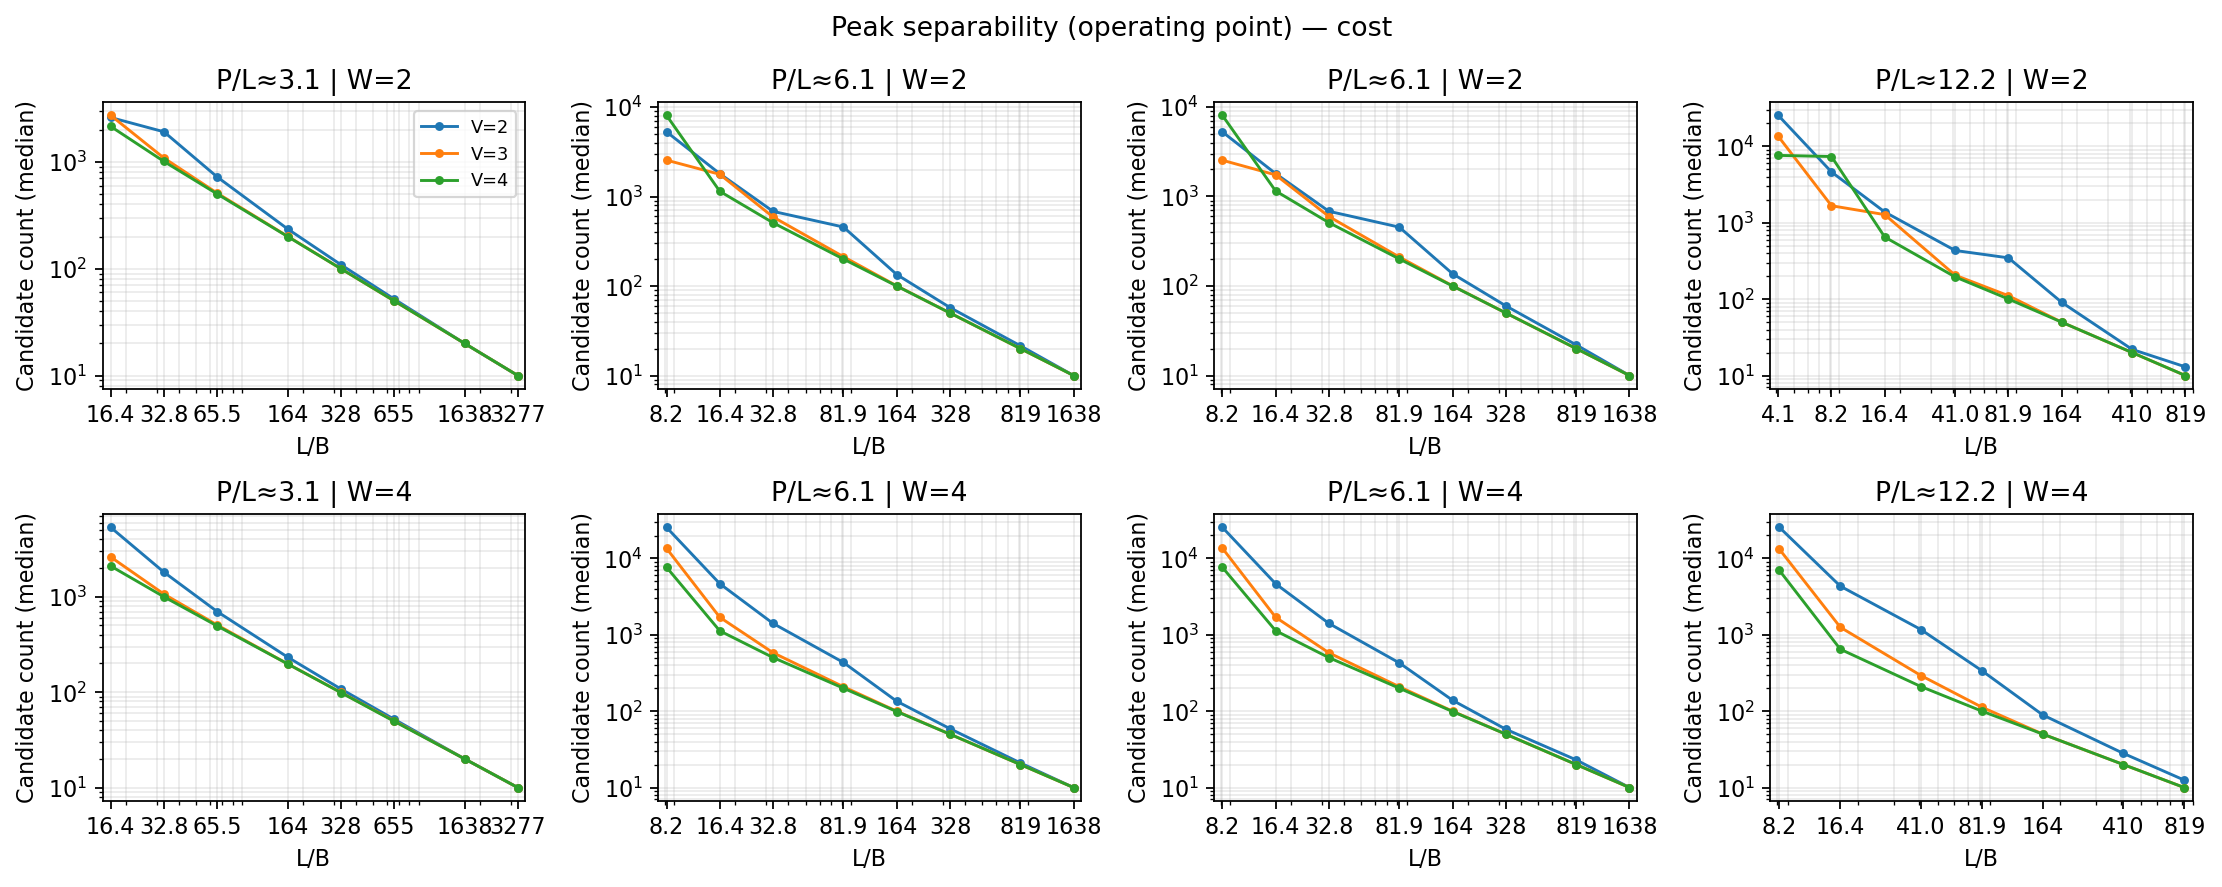
\includegraphics[width=0.9\textwidth]{figures/c4_2_fig_separability_candcnt_med_vs_LoverB.png}
\caption{$L/B$ slices at fixed $P/L$, operating-point \texttt{cand\_cnt} as a function of $L/B$. The three curves in each panel correspond to $V{=}2,3,4$ (blue, orange, and green, respectively). Candidate cost decreases monotonically with increasing $L/B$ across all configurations; larger $V$ yields lower absolute cost at the same $L/B$.}
\label{fig:c4-2}
\end{figure*}

Figure~\ref{fig:c4-a1} extends the parameter range to larger values of $L$. The candidate count \texttt{cand\_cnt} maintains an overall decreasing trend with increasing $L/B$, and the suppression effect of $V$ remains consistent under the extended parameters. For a few panels with $W{=}2$ and $V{=}2$, a plateau or step-like pattern can be observed at the high-$L/B$ end; this phenomenon is related to the discrete selection of operating points: when windows are narrow and the number of views is small, ranking stability is more sensitive, and the discrete grid of \texttt{top\_r} values in the experiment causes the minimum feasible budget to jump between adjacent bins, producing locally non-smooth curves. The curves become smoother with larger $V$ or larger $W$, and the overall trend is unchanged.

\begin{figure*}[!thbp]
\centering
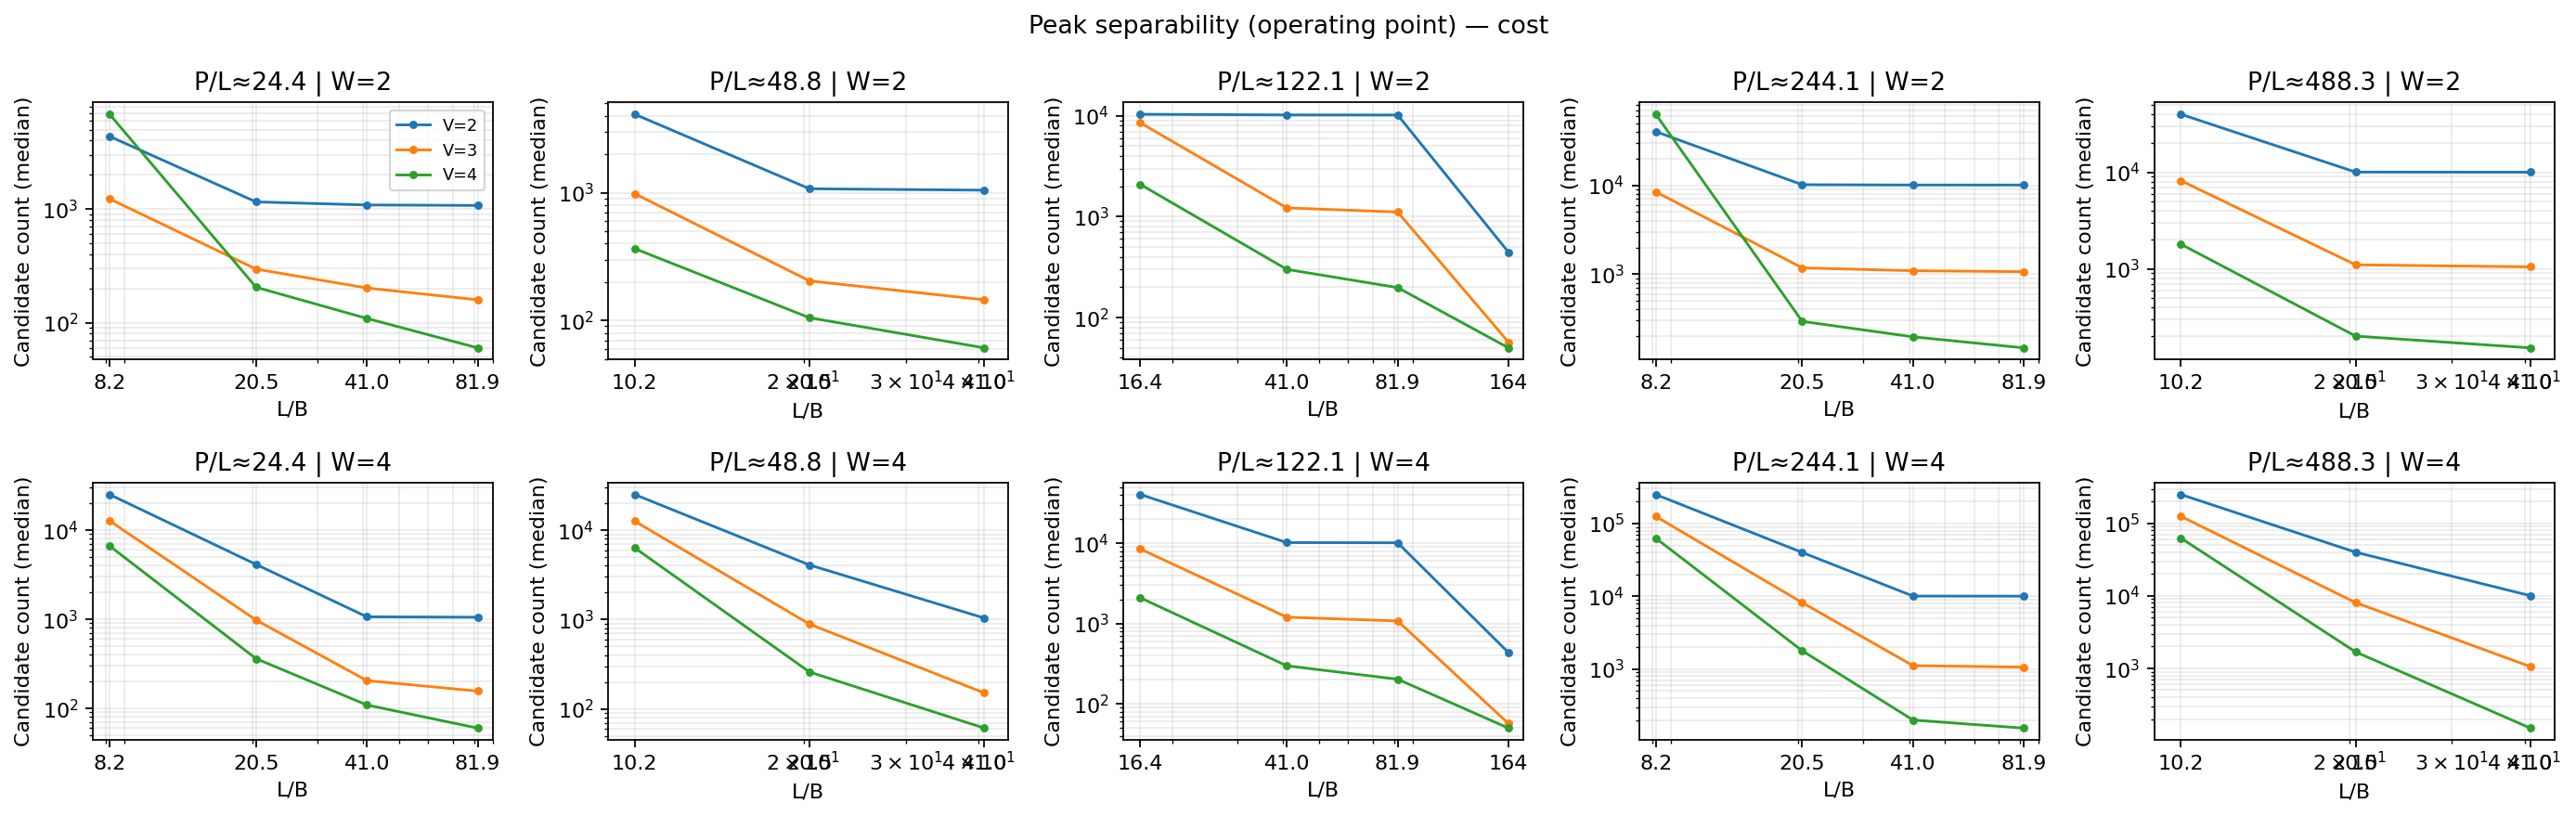
\includegraphics[width=0.9\textwidth]{figures/c4_a1_fig_separability_candcnt_med_vs_LoverB.png}
\caption{Operating-point \texttt{cand\_cnt} (median) as a function of $L/B$ under the extended parameter range. Configuration is the same as the base-range version, but with a wider range of $L$ values. Log scale.}
\label{fig:c4-a1}
\end{figure*}


\subsubsection{$P/L$: Extended Parameter Range}




Figure~\ref{fig:c4-a3} extends the $P/L$ analysis to higher $P/L$ tiers. The candidate count increases monotonically with $P/L$, and the suppression effect of $V$ remains consistent at higher tiers. The tail-risk metric \texttt{halo} (p90) follows exactly the same trend: in this setting it differs from \texttt{cand\_cnt} only by a constant factor on the order of $P/B$, so it is not plotted separately.



\begin{table}[!htbp]
\centering
\small
\begin{tabular}{rrrrr}
\toprule
$P$ & $P/L$ & $V$ & \texttt{cand\_cnt} (med) & \texttt{halo} (p90) \\
\midrule
10{,}000 & 1.2 & 2 & 127 & 1.35 \\
10{,}000{,}000 & 1221 & 2 & 25{,}044 & 251.87 \\
10{,}000{,}000 & 1221 & 4 & 163 & 1.69 \\
\bottomrule
\end{tabular}
\caption{Scale amplification and the suppression effect of $V$ ($L{=}8192$, $W{=}2$, $B{=}10$, \texttt{top\_r}{=}0.05).}
\label{tab:c4-1}
\end{table}


\begin{figure}[!htbp]
\centering
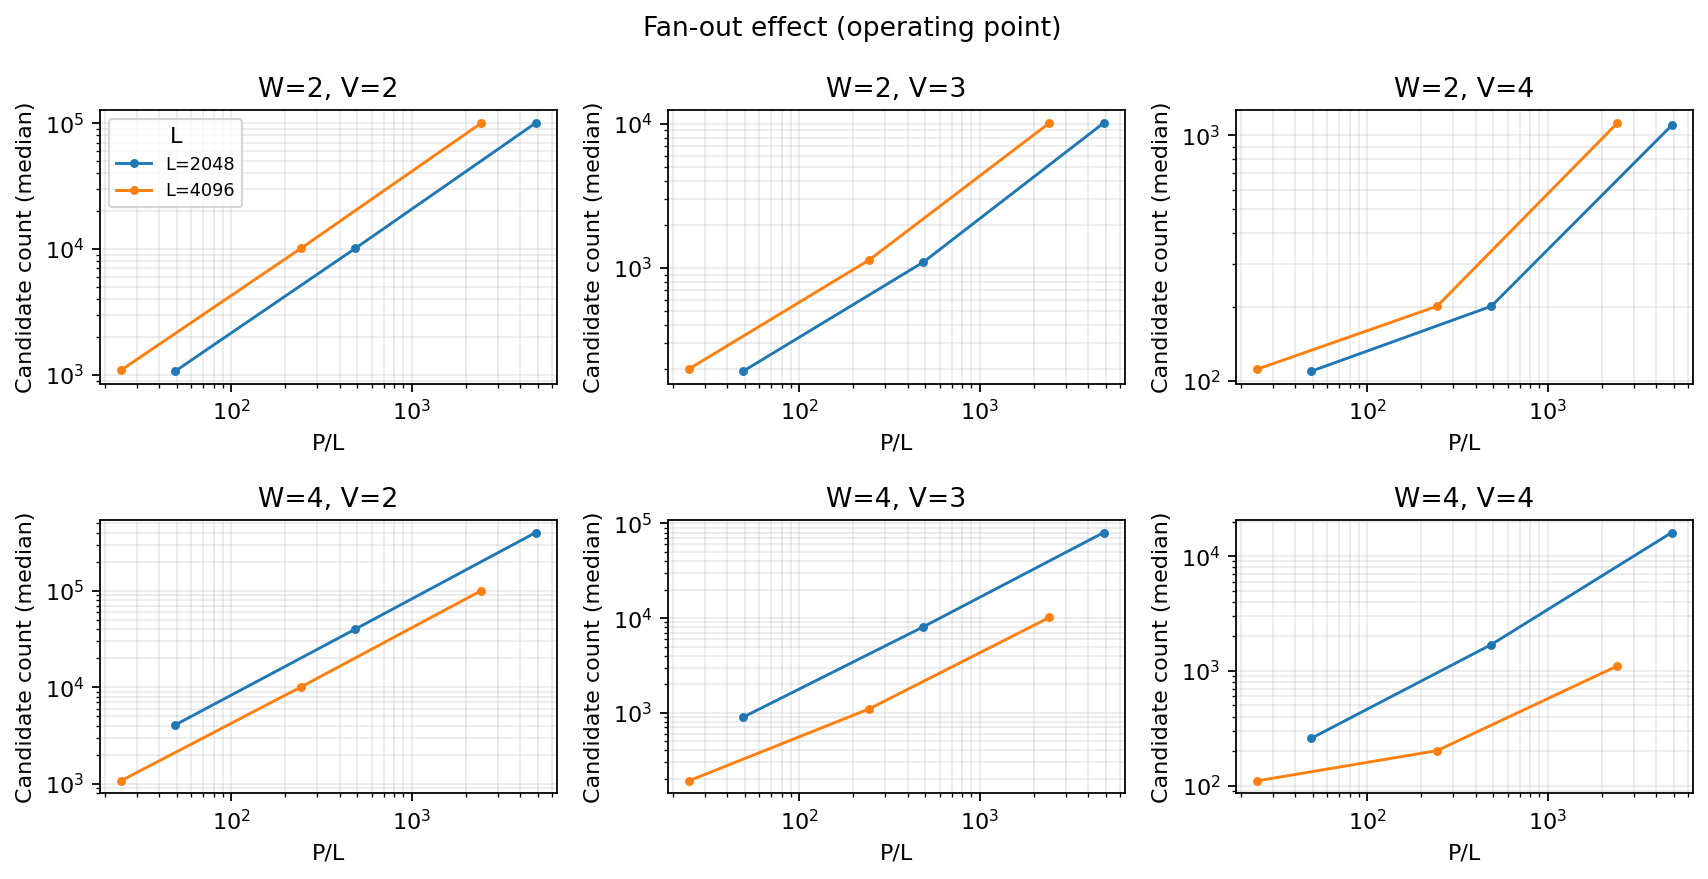
\includegraphics[width=0.9\linewidth]{figures/fig_fanout_candcnt_med_vs_PoverL.png}
\caption{\texttt{cand\_cnt} (median) as a function of $P/L$ under the extended parameter range. Log scale.}
\label{fig:c4-a3}
\end{figure}

\subsection{Theoretical Analysis of Candidate-Set Size and Capacity Threshold Under a Fixed Budget}
\label{sec:appendix-operating-theory}

\label{sec:appendix-budget-alloc}

This subsection studies how a fixed digest budget should be allocated between the number of views $V$ and the section-axis length $L$. Building on the candidate-set framework of Equations~\eqref{eq:cand-expectation} and~\eqref{eq:halo-prob} in the main text, and fixing $m_0{=}32$ as a practical balance between sizing accuracy and memory cost for digest sizing (Supplement~\ref{sec:appendix-sizing-supp}, especially Figure~\ref{fig:c3-a2}), we derive the fixed-budget trade-off between $V$ and $L$, the relaxed-model threshold for when increasing $V$ remains beneficial, and the associated capacity threshold. We then compare these threshold predictions against numerical results. The focus here is offline allocation across cycles; the runtime adaptation of the truncation budget through \texttt{top\_r} is  separately in \S\ref{sec:appendix-stoploss-details}.

\subsubsection{Derivation of the $V$--$L$ Trade-off and Capacity Thresholds}


Within this framework, the candidate set consists of $B$ truly dirty segments and clean segments that are falsely included due to window overlap, whose expected count is $(P{-}B)\,p_{\mathrm{halo}}^V$. The following derivation assumes that $L/B$ is sufficiently large so that the high-energy windows of the $B$ dirty segments are well-dispersed on the section axis and do not compete for top-ranked slots; the number of top windows $t$ required to cover all dirty segments is then of the same order as $BW$, written as $t \approx \alpha BW$, where $\alpha \ge 1$ is a mild inflation factor accounting for ranking redundancy that is approximately 1 within the parameter range of this paper. The failure boundary of this assumption is discussed below.
Here $B$ denotes the number of dirty segments at segment granularity, but in the relaxed model it is  interpreted as an occupancy-scale quantity: it captures how many faults contribute distinct support on the section axis, while weak or highly dispersed discrepancies are absorbed into the effective redundancy factor $\alpha$ rather than inflating $B$ itself.
When heavy-tail noise compresses the ranking margin (\S\ref{sec:eval-comparison}), the effective $\alpha$ can be significantly larger than 1. Since $c\propto \alpha$ in Equation~\eqref{eq:c-def}, an increase in $\alpha$ linearly raises the per-view false-inclusion probability and correspondingly shrinks $V^*=1/(ec)$, thereby proportionally tightening the capacity thresholds of Equations~\eqref{eq:capacity-threshold} (e.g., the threshold becomes $L/B\gtrsim e\alpha W(2W{-}1)$). The closed-form structure itself is unchanged; what changes is the numerical threshold and the scale of the feasible region.


\paragraph{Structure under the budget constraint}

SCOUT's digest budget satisfies
\begin{equation*}
M_{\text{bytes}} = 4\,V\,L\,m_0,
\end{equation*}
so $L = M_{\text{bytes}} / (4Vm_0)$. Substituting this constraint together with $t \approx \alpha BW$ into Equation~\eqref{eq:halo-prob} yields
\begin{equation}\label{eq:phalo-budget}
p_{\text{halo}}(V)
= \min\!\left\{1,\;\frac{\alpha BW(2W{-}1)}{L}\right\}
= \min\!\left\{1,\;cV\right\},
\end{equation}
where
\begin{equation}\label{eq:c-def}
c \;\triangleq\; \frac{4\,\alpha\,B\,W(2W{-}1)\,m_0}{M_{\text{bytes}}}
\end{equation}
is a dimensionless capacity parameter independent of $V$ and $L$. Equation~\eqref{eq:phalo-budget} reveals the core trade-off under a fixed budget: increasing $V$ provides exponential suppression through the intersection term $p_{\mathrm{halo}}^V$, but simultaneously raises the per-view $p_{\mathrm{halo}} = cV$ linearly because the fixed budget forces $L \propto 1/V$. The dominant factor in the false-inclusion term, $(\min\{1,\,cV\})^V$, is determined by the interplay of these two forces.

\paragraph{Threshold for beneficial increases in $V$}

When $cV \ge 1$, $p_{\mathrm{halo}}$ saturates to 1 and the intersection mechanism fails completely---regardless of how large $V$ is, every clean segment is included in the candidate set. Therefore, the meaningful optimization interval is $cV < 1$ (the non-saturated regime). In this regime the $\min$ operator can be dropped, and the false-inclusion factor simplifies to $f(V) = (cV)^V$. Taking the logarithm and differentiating:
\[
\ln f(V) = V\ln(cV),\qquad
\frac{d\ln f}{dV} = \ln(cV) + 1.
\]
Setting the derivative to zero gives the stationary point under continuous relaxation:
$
V^* = \frac{1}{ec}.
$
Since $V$ is a positive integer and the intersection mechanism requires at least two views, the practical condition is $V^* \ge 2$, equivalently 
\begin{equation} \label{eq:c12e}
c \le 1/(2e).
\end{equation}
Although $B$ is generally unknown before diagnosis, this threshold  provides a useful provisioning check: given a provisioned budget $M_{\text{bytes}}$, a conservative estimate $\hat{B}$, and a conservative choice of $\alpha$, evaluating $c$ from Equation~\eqref{eq:c-def} and verifying $V^* \ge 2$ indicates that the budget is large enough, under the relaxed model, for additional views beyond $V{=}2$ to remain potentially beneficial.
Substituting back into $f$ yields the minimum false-inclusion factor predicted by the relaxed model at the continuous optimum:
\begin{equation}\label{eq:fstar}
f(V^*) = \left(\frac{1}{e}\right)^{1/(ec)}
= \exp\!\left(-\frac{M_{\text{bytes}}}
{4e\,\alpha\,B\,W(2W{-}1)\,m_0}\right).
\end{equation}
Equation~\eqref{eq:fstar} expresses how low the relaxed-model prediction can be driven under a fixed total budget as an exponential decay in $M_{\text{bytes}}/B$. As $B$ increases ($c$ increases), the exponent shrinks and the predicted minimum rises; when $c > 1/(2e)$, $V^* < 2$, indicating that under the relaxed model the budget no longer supports beneficial increases beyond the minimum feasible configuration $V{=}2$. 

\paragraph{Feasibility and capacity thresholds}
\label{sec:appendix-feasibility}

Substituting back the original parameters, $cV = \alpha BW(2W{-}1)/L$, so the non-saturation condition $cV < 1$ is equivalent to $L/B > \alpha\,W(2W{-}1)$. This is a necessary but weak condition: it merely prevents $p_{\mathrm{halo}}$ from saturating to~1, but does not guarantee that increasing $V$ is beneficial. The practically useful bound is the \emph{capacity threshold}, which requires $V^* \ge 2$ (Equation~\ref{eq:c12e}) and is a factor of $e$ more stringent:
\begin{equation}\label{eq:capacity-threshold}
\frac{L}{B} \;\gtrsim\; e\,\alpha\,W(2W{-}1).
\end{equation}
Geometrically, this states that the section axis must be long enough to accommodate the coverage footprints and halo neighborhoods of $B$ concurrent faults without driving the per-view halo probability into saturation. Since $L$ is determined by the allocation $L = M_{\text{bytes}}/(4Vm_0)$ rather than chosen independently, the same threshold also serves as a provisioning rule. At the minimum multi-view configuration $V{=}2$, the budget should satisfy
\[
M_{\text{bytes}} \;\gtrsim\; 8e\,\alpha\,B\,W(2W{-}1)\,m_0.
\]
Equivalently, for a fixed budget, the same relaxed threshold implies a planning capacity
\[
B_{\max} \;=\; \frac{M_{\text{bytes}}}{8e\,\alpha\,W(2W{-}1)\,m_0}.
\]
For example, with $W{=}2$, $\alpha{=}1$, and $m_0{=}32$, the threshold gives $L/B \gtrsim 6e \approx 16.3$, and a 512\,KiB digest budget corresponds to $B_{\max} \approx 126$ under the relaxed threshold. The transition band in the main-text heatmap (Figure~\ref{fig:c4-1}) appears at $L/B \sim 10$--$50$, consistent with this order of magnitude.

\paragraph{Role of $P/L$}
\label{sec:appendix-PoverL-role}

The above thresholds are entirely determined by $L/B$ and $W$, while $P$ appears in the derivation only in the coefficient $(P{-}B)$, seemingly amplifying the absolute candidate count only linearly. This conclusion relies on the assumption that $t_{\text{op}} \approx \alpha BW$ does not vary with $P/L$---under a pure bimodal workload (dirty segments have strong signals and the rest are completely clean), the section energy ranking is determined by the dirty-segment signals, so $\alpha \approx 1$ is stable.

When the workload contains significant background noise (e.g., the mixed workloads of \S\ref{sec:eval-comparison}), a higher $P/L$ implies severe hash collisions. A large number of clean segments (as well as slightly dirty ones) spread background energy across the section axis, interfering with the ranking of genuine faults. To ensure that genuinely large faults are not displaced from the candidate list, the system must relax the truncation quota (i.e., the redundancy factor $\alpha$ mentioned above becomes greater than 1).

However, this degradation induced by $P/L$ is mild and gradual: it merely increases the difficulty of ranking, forcing the selection of a few more candidate windows. This is fundamentally different from an increase in the number of concurrent faults $B$---an increase in $B$ physically fills the remaining space on the section axis ($c \propto B$), which saturates the section axis more directly.

\subsubsection{Numerical Verification Under a Fixed Budget}
\label{sec:appendix-isobudget}

Building on Equation~\eqref{eq:halo-prob} in \S\ref{sec:spatial-coupling}, we note that the derivation assumes independently scattered window start positions and therefore yields a conservative relaxed approximation. In practice, the top-ranked high-energy windows tend to cluster tightly around the true faults; the geometric overlap makes the effective halo neighborhood much smaller than the estimate under the independence assumption, so the actual false-inclusion probability is typically lower than this approximation. We next test whether this approximation still provides useful guidance under a fixed budget.

\paragraph{Prediction accuracy of the benefit threshold}

Given a fixed probe budget, increasing $V$ means decreasing $L$. The continuous relaxation above yields the stationary point $V^* = 1/(ec)$ and the corresponding benefit threshold $p_{\mathrm{halo}} = 1/e$. We now test the discriminative power of this threshold under discrete parameters. From the operating-point data of \S\ref{sec:eval-operating}, we pair configurations with the same total budget ($V \cdot L$ fixed) at $V{=}2$ and $V{=}4$, yielding 55 pairs. For each pair, we compute $p_{\mathrm{halo}} = \min\{1,\;t_{\text{op}}(2W{-}1)/L\}$ at the $V{=}2$ operating point and use $p_{\mathrm{halo}} < 1/e$ as the prediction rule for ``increasing $V$ is beneficial,'' then check whether this agrees with the actual change in candidate cost.
After excluding pairs where candidate costs are essentially tied, the rule achieves a prediction accuracy of approximately 90\% among the 41 effective pairs. In terms of absolute values, the formula overestimates by roughly $2\times$ at low $P/L$ and more significantly at high $P/L$ due to clustering effects; however, the discriminative power of the threshold $p_{\mathrm{halo}} = 1/e$ is unaffected, indicating that the scaling laws derived from continuous relaxation remain valid under discrete parameters.

\paragraph{Reversal cases and the asymmetry between $L/B$ and $P/L$}

More informative are the reversal cases---where increasing $V$ while decreasing $L$ worsens candidate cost. Table~\ref{tab:c4-reversal} shows the most prominent example: with $B{=}1000$ and $V{\cdot}L{=}32768$, $p_{\mathrm{halo}} \approx 0.30$ at $V{=}2$ already approaches the benefit threshold. Increasing $V$ to 4 halves $L$ to 8192, saturating $p_{\mathrm{halo}}$ to 1.0 and forcing the operating point to push \texttt{top\_r} to 0.5, inflating candidate cost by roughly $4\times$. This failure path---$V$ increases $\to$ $L$ shrinks $\to$ $p_{\mathrm{halo}}$ saturates $\to$ intersection mechanism fails---is consistent with the saturation mechanism predicted by the relaxed theoretical derivation above.

\begin{table}[!htbp]
\centering
\small
\begin{tabular}{lcccc}
\toprule
& $V$ & $L$ & \texttt{cand\_cnt} (med) \\
\midrule
\multirow{2}{*}{\shortstack[l]{$P{=}10^5$, $B{=}1000$\\$W{=}2$, $VL{=}32768$}}
  & 2 & 16384 &  1799 \\
  & 4 & 8192  &  7377 \\
\midrule
\multicolumn{4}{c}{$p_{\mathrm{halo}}(V{=}2)\approx 0.30$;\quad $p_{\mathrm{halo}}(V{=}4)= 1.00$ (saturated)} & \\
\bottomrule
\end{tabular}
\caption{Fixed-budget reversal example: increasing $V$ from 2 to 4 halves $L$, saturating $p_{\mathrm{halo}}$ to 1.0 and inflating candidate cost by roughly $4\times$.}
\label{tab:c4-reversal}
\end{table}

The asymmetry between the two dimensions is now evident: $L/B$ directly controls the feasibility threshold of the intersection mechanism through $c$ and exhibits a sharp transition around the \textbf{capacity threshold}---once below the threshold, candidate cost degrades sharply and is difficult to compensate; $P/L$, above the threshold, mainly amplifies the absolute candidate count by mildly modifying the effective $c$, and this amplification can be effectively absorbed by the exponential suppression of $V$.



\subsection{Example Verification and Implementation Details for the Runtime Stopping Rule}
\label{sec:appendix-stoploss-details}

This subsection supplements the knee-detection implementation described in \S\ref{sec:eval-operating}, provides post-hoc verification, and derives the resulting runtime fallback rules.

\paragraph{Implementation of knee detection}

The system sweeps upward through a preset \texttt{top\_r} schedule (e.g., $\{10^{-3},\,2\times10^{-3},\,5\times10^{-3},\,10^{-2},\ldots\}$), recording at each step the energy coverage $E_{\mathrm{cdf}}$ (cumulative proportion of section energy ranked in descending order) and the candidate cost $\mathtt{cand\_cnt}$. The joint knee is detected by monitoring the marginal ratio $\Delta E_{\mathrm{cdf}} / \Delta\log(\mathtt{cand\_cnt})$: when this ratio drops significantly below the level of preceding steps, the system declares entry into the diminishing-returns region and terminates expansion.

\paragraph{Post-hoc verification}

Figure~\ref{fig:c4-3-recall} provides offline verification by plotting candidate cost against ground-truth recall (fraction of total diff captured by the candidate set) for each \texttt{top\_r} value. At small \texttt{top\_r}, increasing the truncation budget improves recall at moderate candidate cost; beyond the knee, candidate cost accelerates sharply while recall gains diminish. The knee-based truncation point ($\mathrm{r_{top}}{=}0.25$, dashed reference line) sits at the onset of this diminishing-returns region. This verification requires ground truth and is used only for post-hoc justification; online deployment relies solely on the energy-based signal.


\begin{figure}[!htbp]
\centering
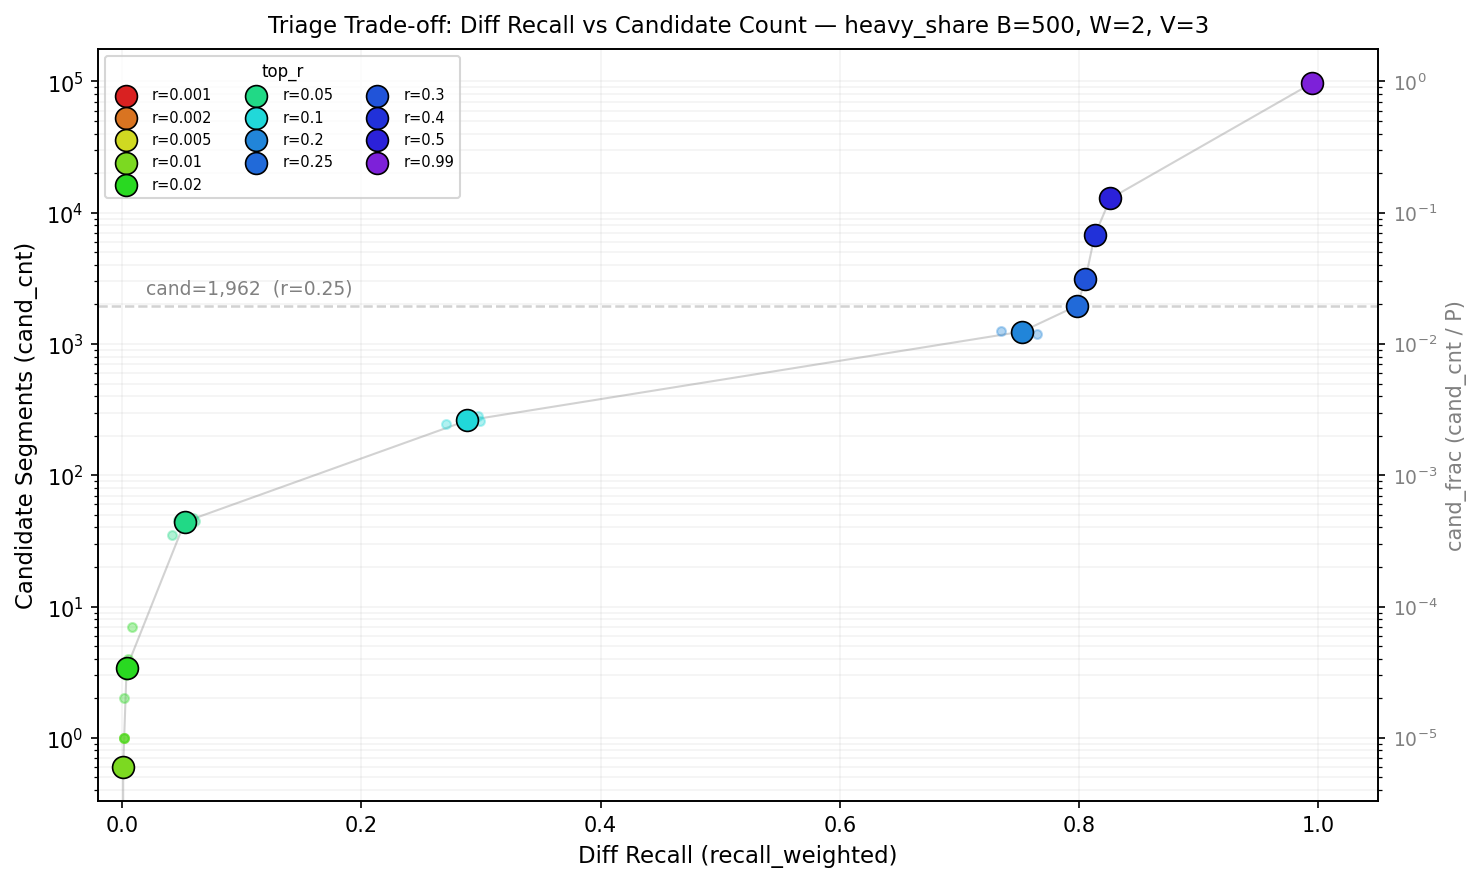
\includegraphics[width=0.95\linewidth]{figures/energy_decay_and_triage_tradeoff.png}
\caption{Recall--cost trade-off for the same configuration as Figure~\ref{fig:c4-knee}. Each colored point corresponds to a \texttt{top\_r} value; the horizontal dashed line marks the knee ($\mathrm{r_{top}}{=}0.25$). Beyond the knee, candidate cost grows rapidly while recall gains diminish.}
\label{fig:c4-3-recall}
\end{figure}
